\chapter{Bioinformatics and Sequence Analysis}\label{ch:b3:bioinformatics}

A biologist who has just sequenced a gene from a deep-sea worm pastes
its \num{300} amino acids into a web form and, three seconds later,
learns that the protein is a distant cousin of a human kinase, with
\qty{31}{\%} identity over \num{280} residues and a probability of
$10^{-40}$ that the resemblance is chance. Behind those three seconds
are a dynamic-programming algorithm from 1970, a statistical theory of
random \omterm{def:b3:bioinformatics:alignment}{alignments}, substitution matrices distilled from thousands of
protein families, and a database of some hundred billion residues.
This chapter is about the reasoning inside the box: how two sequences
are aligned so that the \omterm{def:b3:bioinformatics:alignment}{alignment} is provably the best, how the score
is made to mean something, how a match is told from a coincidence,
and how patterns are found in a genome that no one has looked at
before. The mathematics is elementary --- a recurrence, a logarithm, a
Poisson distribution --- and it is worth knowing, because every
conclusion drawn from a sequence comparison rests on it.

\section{Aligning two sequences}

\begin{definition}[Alignment and score]\label{def:b3:bioinformatics:alignment}
\index{sequence alignment}\index{gap penalty}\index{global alignment}\index{local alignment}
An \emph{alignment} of two sequences writes them one above the other,
with \emph{gaps} (--) inserted so that the columns pair a residue with a
residue or a residue with a gap, and no column pairs two gaps. Its
\emph{score} is the sum over columns of a substitution score $s(a,b)$
for each pair of residues and a \emph{gap penalty} for each gap: a
linear penalty $-d$ per gap position, or, more realistically, an
\emph{affine} penalty $-d - (k-1)e$ for a run of $k$ gaps, with the
opening cost $d$ larger than the extension cost $e$, since one
insertion of several residues is a single evolutionary event. A
\emph{global} alignment covers both sequences end to end; a \emph{local}
alignment finds the highest-scoring pair of substrings and ignores the
rest, which is what one wants when a shared domain sits in two
otherwise unrelated proteins.
\end{definition}

\begin{theorem}[Needleman--Wunsch]\label{thm:b3:bioinformatics:nw}
\index{Needleman--Wunsch}\index{dynamic programming}\index{Smith--Waterman}
Let $x = x_{1}\dots x_{m}$ and $y = y_{1}\dots y_{n}$, with linear \omterm{def:b3:bioinformatics:alignment}{gap
penalty} $d$. Define $F(i,j)$ as the best score of a \omterm{def:b3:bioinformatics:alignment}{global alignment}
of the prefixes $x_{1}\dots x_{i}$ and $y_{1}\dots y_{j}$. Then
$F(i,0) = -id$, $F(0,j) = -jd$, and for $i,j \ge 1$
\[
F(i,j) = \max\bigl\{\,F(i-1,j-1) + s(x_{i},y_{j}),\;
F(i-1,j) - d,\; F(i,j-1) - d\,\bigr\}.
\]
$F(m,n)$ is the optimal global score, an optimal \omterm{def:b3:bioinformatics:alignment}{alignment} is recovered
by tracing back from $(m,n)$ the choices that produced each maximum,
and the whole computation takes $mn$ steps. The \emph{Smith--Waterman}
variant for \omterm{def:b3:bioinformatics:alignment}{local alignment} adds $0$ as a fourth option in the maximum,
sets the borders to $0$, and reads the answer at the largest entry of
the table.
\end{theorem}
\begin{proof}
Consider the last column of any \omterm{def:b3:bioinformatics:alignment}{alignment} of the two prefixes. It is
one of three things: $x_{i}$ over $y_{j}$, $x_{i}$ over a gap, or a gap
over $y_{j}$. Removing it leaves an \omterm{def:b3:bioinformatics:alignment}{alignment} of $(x_{1}\dots x_{i-1},
y_{1}\dots y_{j-1})$, of $(x_{1}\dots x_{i-1}, y_{1}\dots y_{j})$, or of
$(x_{1}\dots x_{i}, y_{1}\dots y_{j-1})$ respectively, whose score is at
most $F$ of that pair; and conversely each of those optimal \omterm{def:b3:bioinformatics:alignment}{alignments}
can be extended by the corresponding last column. So the best score
ending in each kind of column is $F$ of the shorter pair plus the
column's score, and the optimum is the largest of the three. The
borders are forced (only gaps are possible against an empty prefix).
Induction on $i + j$ fills the table; the number of cells is $(m+1)(n+1)$.
For \omterm{def:b3:bioinformatics:alignment}{local alignment} the extra option $0$ means ``start a new \omterm{def:b3:bioinformatics:alignment}{alignment}
here'', which makes $F(i,j)$ the best score of an \omterm{def:b3:bioinformatics:alignment}{alignment} \emph{ending}
at $(i,j)$, and the best \omterm{def:b3:bioinformatics:alignment}{local alignment} ends somewhere.
\end{proof}

\begin{example}[A four-by-three table]\label{ex:b3:bioinformatics:nw-example}
Align GAT with GCAT, scoring $+1$ for a match, $-1$ for a mismatch,
$d = 1$. The borders are $0, -1, -2, -3, -4$ along the top and $0, -1,
-2, -3$ down the side. Filling row by row: $F(\text{G},\text{G}) = 1$,
$F(\text{G},\text{C}) = 0$, $F(\text{G},\text{A}) = -1$,
$F(\text{G},\text{T}) = -2$; $F(\text{A},\text{G}) = 0$,
$F(\text{A},\text{C}) = 0$, $F(\text{A},\text{A}) = 1$,
$F(\text{A},\text{T}) = 0$; $F(\text{T},\text{G}) = -1$,
$F(\text{T},\text{C}) = -1$, $F(\text{T},\text{A}) = 0$,
$F(\text{T},\text{T}) = 2$. The optimum is $2$, and tracing back
--- diagonal from (T,T), diagonal from (A,A), then left from (G,C) to
(G,G), then diagonal --- gives
\[
\begin{array}{c}
\texttt{G-AT}\\
\texttt{GCAT}
\end{array}
\]
three matches and one gap: $3 - 1 = 2$.
\end{example}

\begin{omfigure}
\begin{tikzpicture}[every node/.style={font=\small}, >=stealth]
  \def\dx{1.0}\def\dy{0.8}
  % headers
  \foreach \j/\c in {1/G,2/C,3/A,4/T} \node[omDef, font=\small\bfseries] at (\j*\dx+0.5,0.4) {\c};
  \foreach \i/\c in {1/G,2/A,3/T} \node[omDef, font=\small\bfseries] at (-0.5,-\i*\dy-0.4) {\c};
  % grid
  \draw[gray!60] (0,0) grid[xstep=\dx, ystep=\dy] (5*\dx,-4*\dy);
  % values
  \foreach \i/\j/\v in {0/0/0,0/1/-1,0/2/-2,0/3/-3,0/4/-4,1/0/-1,2/0/-2,3/0/-3, 1/1/1,1/2/0,1/3/-1,1/4/-2, 2/1/0,2/2/0,2/3/1,2/4/0, 3/1/-1,3/2/-1,3/3/0,3/4/2}
    \node at (\j*\dx+0.5,-\i*\dy-0.4) {$\v$};
  % traceback path highlighted
  \foreach \i/\j in {0/0,1/1,1/2,2/3,3/4} \draw[omThm, very thick] (\j*\dx+0.05,-\i*\dy-0.05) rectangle (\j*\dx+\dx-0.05,-\i*\dy-\dy+0.05);
  \draw[->, omThm, very thick, shorten >=8pt, shorten <=8pt] (4.5,-2.8) -- (3.5,-2.0);
  \draw[->, omThm, very thick, shorten >=8pt, shorten <=8pt] (3.5,-2.0) -- (2.5,-1.2);
  \draw[->, omThm, very thick, shorten >=8pt, shorten <=8pt] (2.5,-1.2) -- (1.5,-1.2);
  \draw[->, omThm, very thick, shorten >=8pt, shorten <=8pt] (1.5,-1.2) -- (0.5,-0.4);
  \node[right, align=left] at (5.6,-1.6) {traceback from $F(3,4) = 2$:\\diagonal, diagonal,\\left (gap in GAT), diagonal\\[3pt] \texttt{G-AT}\\\texttt{GCAT}};
\end{tikzpicture}

{\small The Needleman--Wunsch table for GAT against GCAT (match $+1$,
mismatch $-1$, gap $-1$). Each cell is the best score for the two
prefixes ending there; the red path traced back from the corner is the
optimal \omterm{def:b3:bioinformatics:alignment}{alignment}.}
\end{omfigure}

\begin{method}[Aligning two sequences]\label{met:b3:bioinformatics:align}
\index{traceback}
(1) Choose the scoring: a \omterm{def:b3:bioinformatics:matrices}{substitution matrix} suited to the expected
divergence (BLOSUM62 for proteins of unknown distance; match/mismatch
for DNA), and affine gap penalties (typically open $-11$, extend $-1$
with BLOSUM62). (2) Decide global or local: global for two sequences
believed homologous over their whole length, local otherwise.
(3) Fill the table by the recurrence, keeping for each cell a pointer
to the choice that gave its maximum. (4) Trace back from $(m,n)$
(global) or from the maximum cell to a zero (local), writing the
\omterm{def:b3:bioinformatics:alignment}{alignment} from right to left. (5) Judge the result not by its raw
score but by its statistical significance (below), and look at it:
long gaps, low-complexity runs and \omterm{def:b3:bioinformatics:alignment}{alignments} confined to a repeat are
warnings.
\end{method}

\section{Scoring: what a match is worth}

\begin{definition}[Substitution matrices]\label{def:b3:bioinformatics:matrices}
\index{substitution matrix}\index{BLOSUM}\index{PAM}\index{log-odds score}
A \emph{substitution matrix} gives $s(a,b)$ for every pair of amino
acids as a \emph{log-odds score}:
\[
s(a,b) = \frac{1}{\lambda}\,\log\frac{q_{ab}}{p_{a}\,p_{b}},
\]
where $q_{ab}$ is the frequency with which $a$ and $b$ are found
aligned in trusted \omterm{def:b3:bioinformatics:alignment}{alignments} of related proteins, $p_{a} p_{b}$ the
frequency with which they would be paired by chance, and $\lambda$ a
scale chosen to make the entries convenient integers. A positive score
means the pair occurs more often in homologues than by chance; the
identity scores are largest for rare amino acids (tryptophan $+11$,
cysteine $+9$ in BLOSUM62) and smallest for common ones (leucine $+4$,
alanine $+4$), and conservative substitutions (isoleucine--valine $+3$)
score positive while radical ones (tryptophan--glycine $-2$) score
negative. The \emph{PAM} matrices (Dayhoff, 1978) were derived from
closely related proteins and extrapolated to greater distances by
matrix multiplication; the \emph{BLOSUM} matrices (Henikoff and
Henikoff, 1992) were counted directly in blocks of aligned sequences
clustered at a given identity --- BLOSUM62 from blocks at \qty{62}{\%}
--- and are the default because they were measured, not extrapolated,
at the distance where they are used.
\end{definition}

\begin{proposition}[Why log-odds]\label{prop:b3:bioinformatics:logodds}
\index{expected score}
For a scoring scheme to be used in \omterm{def:b3:bioinformatics:alignment}{local alignment}, the \omterm{prop:b3:bioinformatics:logodds}{expected score}
of a randomly paired column, $\sum_{a,b} p_{a} p_{b}\, s(a,b)$, must be
negative, and some scores must be positive; otherwise random
\omterm{def:b3:bioinformatics:alignment}{alignments} would grow without bound and the highest-scoring segment
would be the whole sequence. Given that, any such scheme is
equivalent to a log-odds scheme for \emph{some} target frequencies
$q_{ab}$ --- the \omterm{def:b3:bioinformatics:alignment}{alignments} it will find as optimal are those whose
residue pairs are distributed like $q_{ab}$. Choosing the matrix is
therefore choosing the divergence one expects to detect: a matrix for
close relatives (BLOSUM80, PAM30) has sharper positives and harsher
negatives, one for distant relatives (BLOSUM45, PAM250) is flatter.
\end{proposition}
\admitted

\begin{example}[Identity, similarity and the twilight zone]\label{ex:b3:bioinformatics:twilight}
Two random protein sequences aligned optimally with gaps reach about
\qtyrange{15}{20}{\%} identity by chance. Above \qty{35}{\%} identity
over a hundred residues two proteins are almost surely homologous;
between \qty{20}{\%} and \qty{35}{\%} is the \emph{twilight zone},
where identity alone cannot decide and the statistics below must.
Homologues can fall far below the zone: haemoglobin and myoglobin
subunits share \qty{25}{\%} identity, lysozyme and $\alpha$-lactalbumin
\qty{40}{\%}, and many pairs of proteins with the same fold share less
than \qty{15}{\%}, detectable only by comparing \omterm{def:b3:bioinformatics:msa}{profiles} or structures.
\end{example}

\section{Searching a database}

\begin{definition}[BLAST]\label{def:b3:bioinformatics:blast}
\index{BLAST}\index{seed}\index{high-scoring segment pair}
Aligning a query of \num{300} residues against a database of $10^{11}$
by full \omterm{thm:b3:bioinformatics:nw}{dynamic programming} would take $3\times 10^{13}$ cell updates
per search. \emph{BLAST} (Altschul and colleagues, 1990) trades a little
sensitivity for a thousandfold speed by three steps: (1) list the
query's \emph{words} (three residues for proteins, eleven bases for
DNA) and their high-scoring neighbours; (2) scan the database for
exact word matches --- \emph{seeds}; (3) extend each seed in both
directions without gaps until the score drops a set amount below its
best, keeping the \emph{high-scoring segment pairs} (HSPs), then join
nearby HSPs with gapped \omterm{thm:b3:bioinformatics:nw}{dynamic programming} in a narrow band. A true
homologue almost always contains at least one exact three-residue
word in common; a chance resemblance rarely does, and is never
extended.
\end{definition}

\begin{omfigure}
\begin{tikzpicture}[every node/.style={font=\scriptsize}, >=stealth]
  % query and database sequences as bars
  \draw[very thick, omDef] (0,2.0) -- (5,2.0); \node[left] at (-0.1,2.0) {query};
  \draw[very thick, gray] (0,0.6) -- (11,0.6); \node[left] at (-0.1,0.6) {database};
  % seeds
  \foreach \q/\d in {1.2/3.6, 2.8/5.2, 4.1/9.3} {
    \fill[omThm] (\q-0.15,1.9) rectangle (\q+0.15,2.1);
    \fill[omThm] (\d-0.15,0.5) rectangle (\d+0.15,0.7);
    \draw[omThm, thick] (\q,1.85) -- (\d,0.75);
  }
  \node[above] at (1.2,2.15) {word}; \node[above] at (2.8,2.15) {word}; \node[above] at (4.1,2.15) {word};
  % extension of the first two (same diagonal) -> HSP
  \draw[<->, very thick, omMeth!70!black] (2.6,0.3) -- (6.2,0.3); \node[below] at (4.4,0.25) {extend without gaps: an HSP};
  % third seed: extension fails
  \draw[omProp, thick, dashed] (8.8,0.3) -- (9.8,0.3); \node[below, omProp] at (9.3,0.25) {score falls: dropped};
  \node[right, align=left] at (5.5,2.0) {1. words of the query\\2. exact hits in the database (seeds)\\3. extend, keep high-scoring pairs};
\end{tikzpicture}

{\small The \omterm{def:b3:bioinformatics:blast}{BLAST} heuristic. Short exact words shared by query and
database entry (red) are \omterm{def:b3:bioinformatics:blast}{seeds}; each is extended along its diagonal
while the score keeps rising, and only extensions that stay high become
\omterm{def:b3:bioinformatics:blast}{high-scoring segment pairs}.}
\end{omfigure}

\begin{theorem}[The statistics of a random hit]\label{thm:b3:bioinformatics:evalue}
\index{E-value}\index{bit score}\index{Karlin--Altschul}
For a query of length $m$ searched against a database of total length
$n$, with a scoring scheme of negative \omterm{prop:b3:bioinformatics:logodds}{expected score}, the number of
ungapped \omterm{def:b3:bioinformatics:alignment}{local alignments} scoring at least $S$ that arise by chance is
Poisson-distributed with mean
\[
E = K\,m\,n\,e^{-\lambda S},
\]
where $\lambda$ and $K$ depend only on the scoring scheme and the
residue frequencies ($\lambda$ is the scale of the log-odds matrix).
$E$ is the \emph{expect value} of the score $S$. Writing the score in
\emph{bits}, $S' = (\lambda S - \ln K)/\ln 2$, the formula becomes
$E = m n\, 2^{-S'}$, and the probability that at least one chance
\omterm{def:b3:bioinformatics:alignment}{alignment} reaches $S$ is $P = 1 - e^{-E}$, which equals $E$ when $E$
is small.
\end{theorem}
\begin{proof}[Partial proof]
The exponential tail is the Karlin--Altschul theorem and is admitted:
the maximal segment score of a random walk with negative drift has a
distribution whose tail decays as $e^{-\lambda S}$, with $\lambda$ the
positive root of $\sum_{a,b} p_{a} p_{b} e^{\lambda s(a,b)} = 1$ ---
which is exactly the equation that makes the log-odds matrix consistent.
Given that tail, the rest is counting. High-scoring segments can start
at any of the $mn$ pairs of positions, they are rare, and they are
nearly independent; the number of them exceeding $S$ is therefore
Poisson with a mean proportional to $mn$ and to the tail probability,
$E = Kmn\,e^{-\lambda S}$. The probability of none is $e^{-E}$. The
bit-score substitution is algebra: $e^{-\lambda S} K = 2^{-(\lambda S -
\ln K)/\ln 2}$. For gapped \omterm{def:b3:bioinformatics:alignment}{alignments} the same form holds with $\lambda$
and $K$ estimated by simulation.
\end{proof}

\begin{example}[Reading an E-value]\label{ex:b3:bioinformatics:evalue}
A query of \num{250} residues against a database of $5\times 10^{10}$
residues has $mn = 1.25\times 10^{13} \approx 2^{43.5}$. A hit with a
\omterm{thm:b3:bioinformatics:evalue}{bit score} of $60$ has $E = 2^{43.5 - 60} = 2^{-16.5} \approx 10^{-5}$:
essentially certainly a homologue. A hit with $S' = 40$ has $E = 2^{3.5}
\approx 11$: eleven such scores are expected by chance, and the hit
means nothing. The \emph{same} \omterm{def:b3:bioinformatics:alignment}{alignment}, with the same \omterm{thm:b3:bioinformatics:evalue}{bit score},
searched against a database ten times larger, has an $E$ ten times
larger --- significance is a property of the search, not of the pair.
The threshold in common use is $E < 10^{-3}$ for a confident homologue;
$E \approx 0.01$--$1$ deserves a second look with a \omterm{def:b3:bioinformatics:msa}{profile} method.
\end{example}

\begin{omfigure}
\begin{tikzpicture}
\begin{axis}[
  width=0.7\linewidth, height=5.6cm,
  axis x line=bottom, axis y line=left,
  xmin=25, xmax=70, ymin=0.000000001, ymax=100000000, ymode=log,
  xlabel={bit score $S'$}, ylabel={$E$},
  xlabel style={font=\small, at={(axis description cs:0.5,-0.12)}, anchor=north},
  ylabel style={font=\small},
  tick label style={font=\small}, xtick={30,40,50,60,70},
  clip=false,
]
\addplot[very thick, omDef, domain=25:70, samples=2] {2^(43.5-x)};
\addplot[very thick, omThm, domain=25:70, samples=2] {2^(46.8-x)};
\addplot[dashed, gray, domain=25:70, samples=2] {0.001};
\node[font=\scriptsize, gray, anchor=south west] at (axis cs:25.5,0.0012) {$E = 10^{-3}$};
\node[font=\scriptsize, omDef, anchor=north west] at (axis cs:26,0.00002) {$mn = 1.25\times 10^{13}$};
\node[font=\scriptsize, omThm, anchor=south west] at (axis cs:45,30) {$mn$ ten times larger};
\end{axis}
\end{tikzpicture}

{\small $E = mn\,2^{-S'}$: each extra bit halves the expected number
of chance hits, and a tenfold larger database costs $3.3$ bits of
significance for the same \omterm{def:b3:bioinformatics:alignment}{alignment}.}
\end{omfigure}

\section{Profiles, hidden states and motifs}

\begin{definition}[Multiple alignment and profiles]\label{def:b3:bioinformatics:msa}
\index{multiple sequence alignment}\index{profile}\index{profile hidden Markov model}
A \emph{multiple \omterm{def:b3:bioinformatics:alignment}{sequence alignment}} arranges a family of sequences in
columns of homologous residues. Exact \omterm{thm:b3:bioinformatics:nw}{dynamic programming} over $k$
sequences costs $n^{k}$ and is impossible beyond three; practical
programs align \emph{progressively}, first the closest pair by a guide
tree, then sequences and groups to the growing \omterm{def:b3:bioinformatics:alignment}{alignment}, with rounds
of refinement. A finished \omterm{def:b3:bioinformatics:alignment}{alignment} is summarised as a \emph{profile}:
for each column, the frequency of each residue and of gaps. A
\emph{profile hidden Markov model} formalises this as a chain of match
states, one per conserved column, each emitting residues with its own
probabilities, with insert and delete states allowing extra or missing
residues at each position; the model of a family (a Pfam entry) scores
a new sequence by the probability of the best path through the states,
and finds homologues far below the twilight zone of pairwise
comparison, because a column that tolerates only hydrophobic residues
says so, while a single sequence cannot.
\end{definition}

\begin{omfigure}
\begin{tikzpicture}[every node/.style={font=\scriptsize}, >=stealth]
  % match states
  \foreach \i in {1,2,3,4} { \draw[thick, fill=omDef!25] (2.2*\i-0.5,0) rectangle (2.2*\i+0.5,0.7); \node at (2.2*\i,0.35) {M$_{\i}$}; }
  % insert states (diamonds) above
  \foreach \i in {1,2,3} { \draw[thick, fill=omProp!30] (2.2*\i+1.1,1.6) -- (2.2*\i+1.55,2.05) -- (2.2*\i+1.1,2.5) -- (2.2*\i+0.65,2.05) -- cycle; \node at (2.2*\i+1.1,2.05) {I$_{\i}$}; }
  % delete states (circles) below
  \foreach \i in {2,3} { \draw[thick, fill=gray!20] (2.2*\i,-1.3) circle (0.4); \node at (2.2*\i,-1.3) {D$_{\i}$}; }
  % transitions match->match
  \foreach \i in {1,2,3} \draw[->, thick] (2.2*\i+0.5,0.35) -- (2.2*\i+1.7,0.35);
  % match->insert->match
  \foreach \i in {1,2,3} { \draw[->, thick, omProp] (2.2*\i+0.3,0.7) -- (2.2*\i+0.9,1.65); \draw[->, thick, omProp] (2.2*\i+1.3,1.65) -- (2.2*\i+1.9,0.7); \draw[->, thick, omProp] (2.2*\i+1.1,2.5) arc[start angle=200, end angle=-20, radius=0.3]; }
  % match->delete->match
  \draw[->, thick, gray] (2.2+0.3,0) -- (4.4-0.3,-1.0); \draw[->, thick, gray] (4.4+0.3,-1.0) -- (6.6-0.3,0); \draw[->, thick, gray] (4.4+0.4,-1.3) -- (6.6-0.4,-1.3); \draw[->, thick, gray] (6.6+0.3,-1.0) -- (8.8-0.3,0);
  \node[below, align=center] at (2.2,-1.2) {emissions: one residue\\distribution per match state};
  \node[right, align=left] at (9.6,1.2) {a sequence scores by\\its best path: matches,\\inserts (orange) and\\deletions (grey)};
\end{tikzpicture}

{\small A \omterm{def:b3:bioinformatics:msa}{profile hidden Markov model} of a four-column family. Each
match state M emits a residue with the column's own frequencies;
insert states I (with self-loops) admit extra residues, delete states D
skip a column. Scoring a sequence is finding its most probable path.}
\end{omfigure}

\begin{definition}[Motifs and information content]\label{def:b3:bioinformatics:motif}
\index{motif}\index{position weight matrix}\index{information content}\index{sequence logo}
A \emph{motif} is a short pattern --- a transcription-factor site, a
splice signal, a phosphorylation site --- represented by a
\emph{position weight matrix} of the frequency $f_{i}(b)$ of each base
or residue $b$ at each position $i$. The \emph{information content} of
position $i$ is $R_{i} = 2 - H_{i}$ bits for DNA, where $H_{i} =
-\sum_{b} f_{i}(b)\log_{2} f_{i}(b)$ is its entropy: $2$ bits for an
invariant base, $0$ for a position where all four are equally likely.
The total $R = \sum_{i} R_{i}$ is drawn as a \emph{sequence logo}, each
position a stack of letters whose total height is $R_{i}$ and whose
letters are sized by frequency.
\end{definition}

\begin{proposition}[How much information a site needs]\label{prop:b3:bioinformatics:bits}
\index{information content!and genome size}
A site that must be found $\gamma$ times in a genome of $G$ positions,
and nowhere else, needs about $R_{\text{needed}} = \log_{2}(G/\gamma)$
bits of \omterm{def:b3:bioinformatics:motif}{information content}: the \omterm{def:b3:bioinformatics:motif}{motif} must reduce the $G$ candidate
positions to the $\gamma$ true ones, and each bit halves the
candidates. Observed \omterm{def:b3:bioinformatics:motif}{motifs} of well-studied bacterial regulators match
this prediction --- \emph{E.~coli} sites for a repressor binding a few
dozen places in a \qty{4.6}{Mb} genome carry \numrange{16}{18} bits;
eukaryotic transcription-factor \omterm{def:b3:bioinformatics:motif}{motifs}, at \numrange{8}{12} bits in a
$3\times 10^{9}$ genome, cannot specify their targets alone, which is
why they act in combinations and in the open \omterm{def:b3:chromatin-epigenetics:nucleosome}{chromatin} of
\cref{ch:b3:chromatin-epigenetics}.
\end{proposition}
\begin{proof}
A random position matches a \omterm{def:b3:bioinformatics:motif}{motif} of \omterm{def:b3:bioinformatics:motif}{information content} $R$ with
probability about $2^{-R}$ (each bit of specificity halves the chance),
so the expected number of chance matches in $G$ positions is $G\,2^{-R}$.
For the true sites to stand out this must be of order $\gamma$ or less:
$G\,2^{-R} \le \gamma$, that is, $R \ge \log_{2}(G/\gamma)$.
\end{proof}

\begin{example}[Expected chance matches]\label{ex:b3:bioinformatics:motif-numbers}
A restriction site of six fixed bases has $R = 12$ bits and matches a
random position with probability $4^{-6} = 2^{-12}$: about \num{1100}
times in an \emph{E.~coli} genome of \qty{4.6}{Mb} read on both strands
(the site is palindromic, so once per position), and $7\times 10^{5}$
times in the human genome. A eukaryotic factor whose \omterm{def:b3:bioinformatics:motif}{motif} carries
$10$ bits matches $3\times 10^{9}\times 2^{-10} \approx 3$ million
positions in the human genome, several thousand times more than the
genes it regulates. A \omterm{def:b3:bioinformatics:motif}{motif} alone is a weak predictor in a large
genome; the \omterm{def:b3:chromatin-epigenetics:nucleosome}{chromatin} state, the neighbouring \omterm{def:b3:bioinformatics:motif}{motifs} and the
conservation of the site across species are what make a prediction.
\end{example}

\begin{omfigure}
\begin{tikzpicture}[every node/.style={font=\scriptsize}]
  % sequence logo: TATA box-like 8 positions, stack heights = information content (1 bit = 1 cm)
  \draw[->] (0,0) -- (0,2.2); \node[left] at (-0.05,2.0) {2}; \node[left] at (-0.05,1.0) {1}; \node[left] at (-0.05,0) {0}; \node[rotate=90, above] at (-0.55,1.1) {bits};
  \draw (0,0) -- (8.6,0);
  \node[anchor=south, inner sep=0] at (0.5,0) {\resizebox{0.6cm}{1.9cm}{\textcolor{omThm}{\bfseries T}}};
  \node[anchor=south, inner sep=0] at (1.5,0) {\resizebox{0.6cm}{1.9cm}{\textcolor{omMeth!70!black}{\bfseries A}}};
  \node[anchor=south, inner sep=0] at (2.5,0) {\resizebox{0.6cm}{1.7cm}{\textcolor{omThm}{\bfseries T}}};
  \node[anchor=south, inner sep=0] at (3.5,0) {\resizebox{0.6cm}{1.9cm}{\textcolor{omMeth!70!black}{\bfseries A}}};
  \node[anchor=south, inner sep=0] at (4.5,0) {\resizebox{0.6cm}{1.0cm}{\textcolor{omMeth!70!black}{\bfseries A}}};
  \node[anchor=south, inner sep=0] at (4.5,1.0) {\resizebox{0.6cm}{0.4cm}{\textcolor{omThm}{\bfseries T}}};
  \node[anchor=south, inner sep=0] at (5.5,0) {\resizebox{0.6cm}{1.3cm}{\textcolor{omMeth!70!black}{\bfseries A}}};
  \node[anchor=south, inner sep=0] at (5.5,1.3) {\resizebox{0.6cm}{0.3cm}{\textcolor{omThm}{\bfseries T}}};
  \node[anchor=south, inner sep=0] at (6.5,0) {\resizebox{0.6cm}{0.5cm}{\textcolor{omProp}{\bfseries G}}};
  \node[anchor=south, inner sep=0] at (6.5,0.5) {\resizebox{0.6cm}{0.3cm}{\textcolor{omMeth!70!black}{\bfseries A}}};
  \node[anchor=south, inner sep=0] at (7.5,0) {\resizebox{0.6cm}{0.3cm}{\textcolor{omProp}{\bfseries G}}};
  \foreach \i in {1,...,8} \node[below] at (\i-0.5,-0.05) {\i};
  \node[below] at (4.3,-0.5) {position in the site};
\end{tikzpicture}

{\small A \omterm{def:b3:bioinformatics:motif}{sequence logo} of a TATA-box-like promoter \omterm{def:b3:bioinformatics:motif}{motif}. The height
of each stack is the \omterm{def:b3:bioinformatics:motif}{information content} of that position, $2 - H_{i}$
bits; the first four positions are nearly invariant and carry most of
the \omterm{def:b3:bioinformatics:motif}{motif}'s $12$ bits or so.}
\end{omfigure}

\section{From sequence to function}

\begin{method}[Annotating an unknown protein]\label{met:b3:bioinformatics:annotate}
\index{domain}\index{orthology inference}
Given a new coding sequence: (1) translate it in the right frame and
check for a signal peptide, transmembrane segments and low-complexity
regions; (2) search the protein databases with \omterm{def:b3:bioinformatics:blast}{BLAST} and read the hits
with $E < 10^{-3}$, noting whether the \omterm{def:b3:bioinformatics:alignment}{alignment} covers the whole
protein (a true \omterm{def:b3:genomics:comparative}{ortholog}) or a segment (a shared domain); (3) search
the domain databases with \omterm{def:b3:bioinformatics:msa}{profile} HMMs, which find families that \omterm{def:b3:bioinformatics:blast}{BLAST}
misses and partition the protein into domains; (4) infer orthology, not
merely similarity, by checking that the best hit in the other genome
has the query as \emph{its} best hit (reciprocal best hits) or by
placing the protein in a gene tree (\cref{ch:b3:molecular-evolution});
(5) transfer the function of \omterm{def:b3:genomics:comparative}{orthologs} with caution --- a conserved
catalytic residue argues for conserved chemistry, a missing one against
--- and predict the structure; (6) treat every prediction as a
hypothesis for the bench.
\end{method}

\begin{proposition}[Structure from sequence]\label{prop:b3:bioinformatics:structure}
\index{structure prediction}\index{homology modelling}\index{coevolution}
A protein's fold is determined by its sequence
(\cref{ch:b3:structural-biology}), and computing it from the sequence
was for fifty years the central unsolved problem of the field. Three
approaches succeeded in turn. \emph{\omterm{prop:b3:bioinformatics:structure}{Homology modelling}} builds the
structure of a protein on that of a solved homologue, reliably above
\qty{30}{\%} identity. \emph{Coevolution analysis} exploits the fact
that two residues in contact in the fold tend to mutate together
across a deep multiple \omterm{def:b3:bioinformatics:alignment}{alignment}, so that statistically coupled pairs
of columns are predicted contacts, and enough contacts define a fold.
Deep-learning methods trained on the hundred thousand solved
structures and on such \omterm{def:b3:bioinformatics:alignment}{alignments} now predict most globular protein
structures to near-experimental accuracy (the CASP assessments of
2020), and databases hold a predicted structure for essentially every
known protein sequence. What they predict less well is what a single
structure does not capture: disordered regions, alternative
conformations, the effect of a point mutation, and complexes.
\end{proposition}

\begin{omfigure}
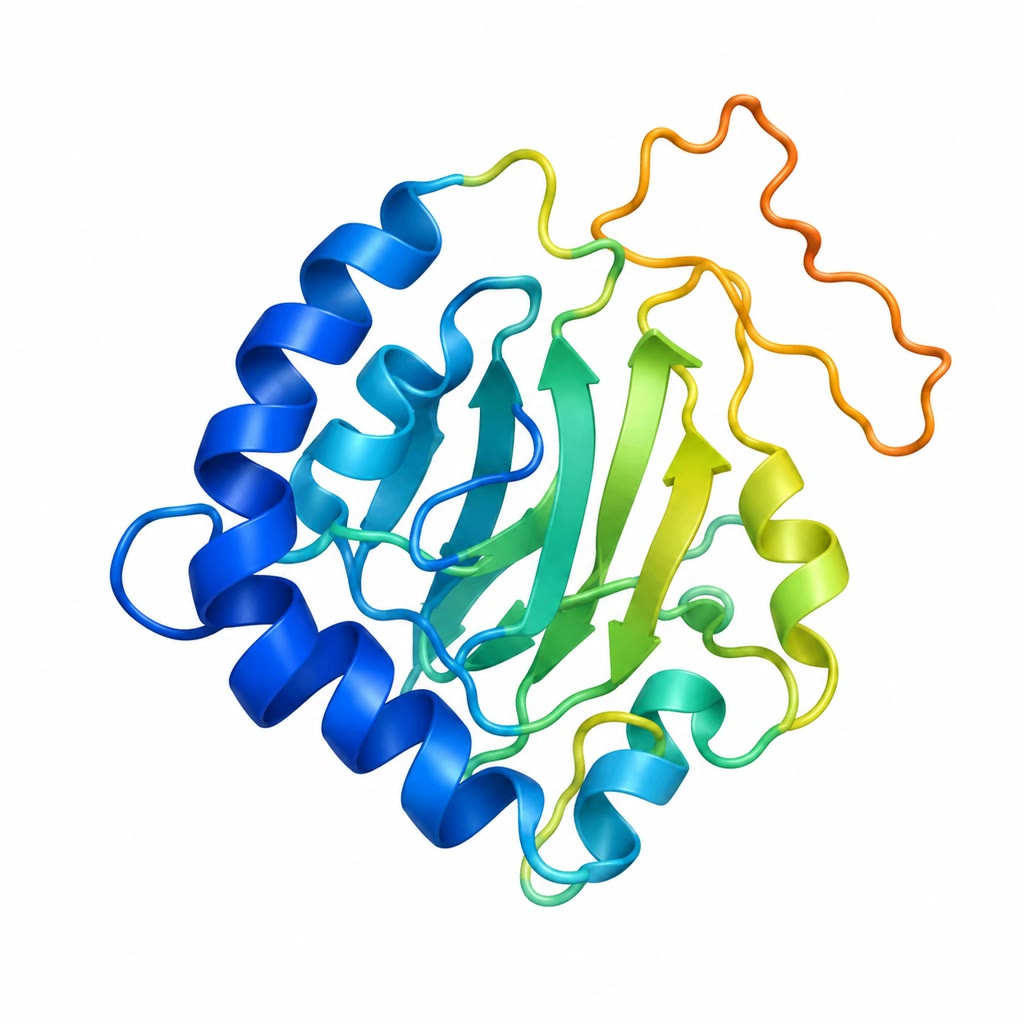
\includegraphics[width=0.36\linewidth]{images/book5/ai/b5-05-alphafold.jpg}\hspace{0.04\linewidth}
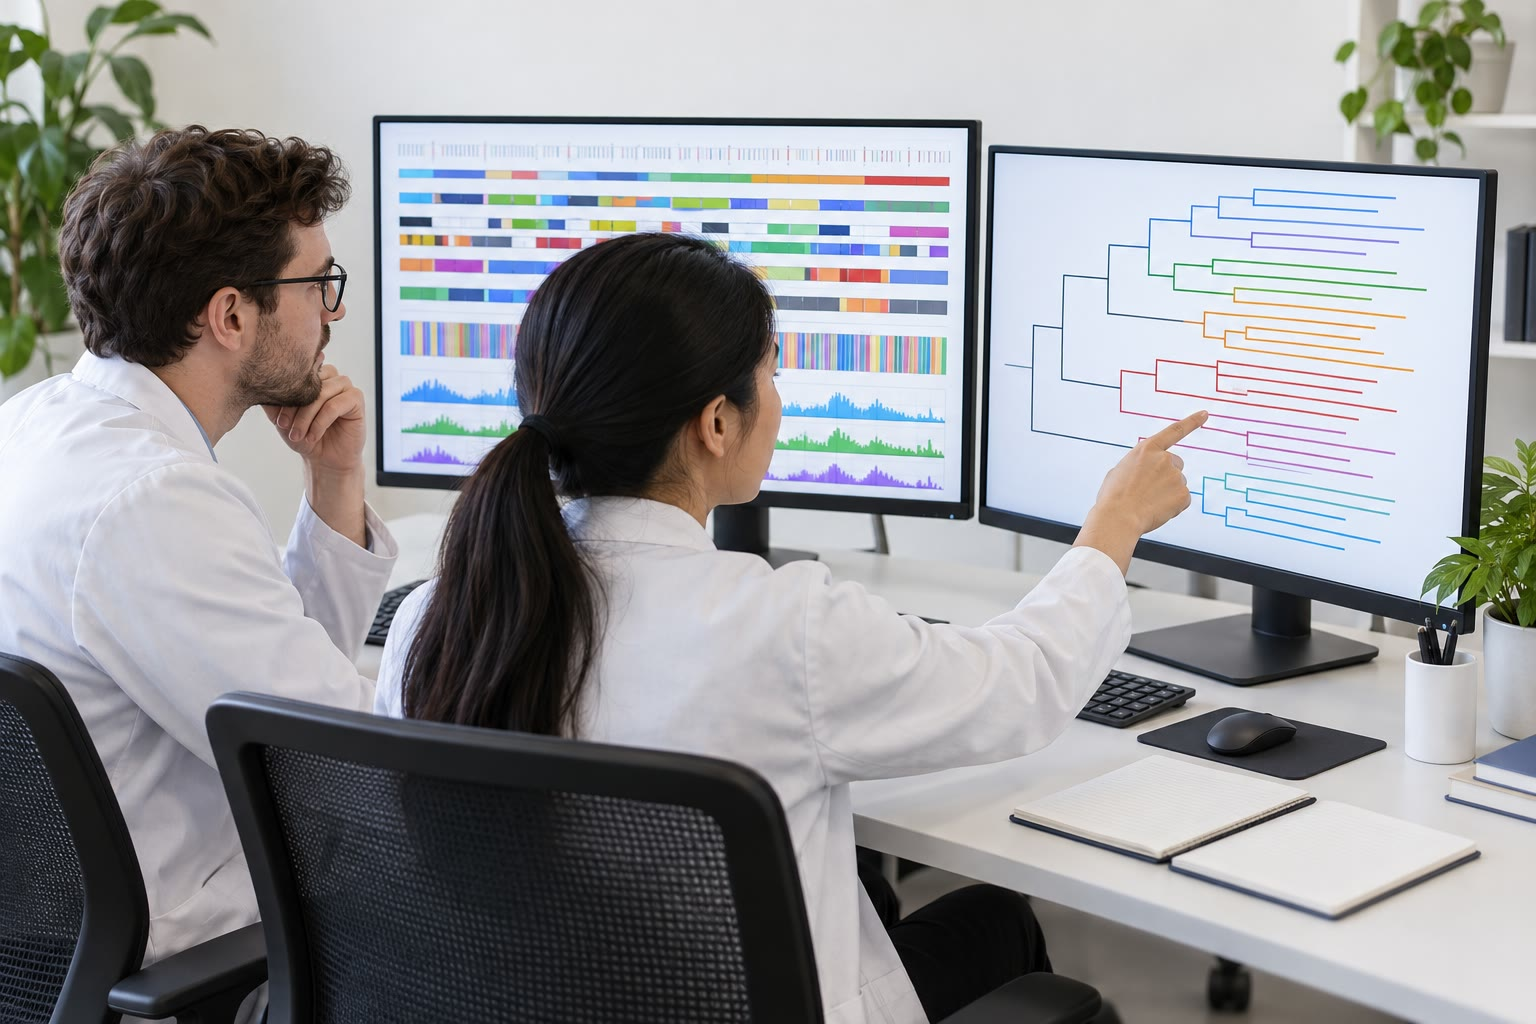
\includegraphics[width=0.54\linewidth]{images/book5/ai/b5-05-bioinformatics-lab.jpg}

{\small Left: a predicted protein structure, coloured by the model's
confidence from high (blue) to low (orange) in a disordered loop.
Right: a bioinformatics office --- genome browsers and trees on the
screens, and no wet bench in sight.}
\end{omfigure}

\begin{remark}[The limits of inference]\label{rem:b3:bioinformatics:limits}
Most functional \omterm{def:b3:genomics:assembly}{annotations} in the databases were never tested; they
were transferred from a homologue, which had in turn been annotated by
transfer. Errors propagate and multiply, and a wrong \omterm{def:b3:genomics:assembly}{annotation} on a
well-connected protein can infect a whole family. The remedies are the
ones above: distinguish orthology from homology, read the \omterm{def:b3:bioinformatics:alignment}{alignment},
look for the catalytic residues, and remember that ``hypothetical
protein'' is an honest label that a third of the genes in most genomes
still deserve.
\end{remark}

\section{Exercises}

\begin{exercise}[$\star$]\label{exo:b3:bioinformatics:1}
Define global and \omterm{def:b3:bioinformatics:alignment}{local alignment} and give one biological situation
that calls for each.
\end{exercise}

\begin{exercise}[$\star$]\label{exo:b3:bioinformatics:2}
Fill the Needleman--Wunsch table for AGC against AAC with match $+1$,
mismatch $-1$, gap $-1$, and give the optimal \omterm{def:b3:bioinformatics:alignment}{alignment} and score.
\end{exercise}

\begin{exercise}[$\star$]\label{exo:b3:bioinformatics:3}
In BLOSUM62, tryptophan--tryptophan scores $+11$ and leucine--leucine
$+4$. Explain from the log-odds formula why the rarer residue's
identity is worth more.
\end{exercise}

\begin{exercise}[$\star$]\label{exo:b3:bioinformatics:4}
What is an E-value? A search returns a hit with $E = 3$. What does that
number mean, and is the hit a homologue?
\end{exercise}

\begin{exercise}[$\star\star$]\label{exo:b3:bioinformatics:5}
A query of \num{400} residues is searched against $2\times 10^{11}$
residues. Compute the E-value of hits with \omterm{thm:b3:bioinformatics:evalue}{bit scores} $45$, $55$ and
$65$. Which \omterm{thm:b3:bioinformatics:evalue}{bit score} gives $E = 10^{-3}$? How does the answer change
if the query is \num{40} residues long?
\end{exercise}

\begin{exercise}[$\star\star$]\label{exo:b3:bioinformatics:6}
Compute the \omterm{def:b3:bioinformatics:motif}{information content} of a \omterm{def:b3:bioinformatics:motif}{motif} whose four positions have
base frequencies (A, C, G, T) of $(1,0,0,0)$, $(0.5,0,0.5,0)$,
$(0.25,0.25,0.25,0.25)$ and $(0.7,0.1,0.1,0.1)$. How many chance
matches does it have in a \qty{4.6}{Mb} genome?
\end{exercise}

\begin{exercise}[$\star\star$]\label{exo:b3:bioinformatics:7}
Explain why affine gap penalties are more realistic than linear ones,
and why a very high gap-opening penalty and a very low one both give
poor \omterm{def:b3:bioinformatics:alignment}{alignments}.
\end{exercise}

\begin{exercise}[$\star\star$]\label{exo:b3:bioinformatics:8}
A \omterm{def:b3:bioinformatics:blast}{BLAST} search of a human protein against a fly database gives a best
hit with $E = 10^{-30}$ covering residues 50--180 of the
\num{600}-residue query. Is the fly protein the \omterm{def:b3:genomics:comparative}{ortholog} of the human
one? What further test would you do?
\end{exercise}

\begin{exercise}[$\star\star$]\label{exo:b3:bioinformatics:9}
Why do \omterm{def:b3:bioinformatics:msa}{profile} methods detect homologues that pairwise \omterm{def:b3:bioinformatics:alignment}{alignment}
misses? Give an example of a column pattern that a \omterm{def:b3:bioinformatics:msa}{profile} captures
and a single sequence cannot.
\end{exercise}

\begin{exercise}[$\star\star\star$]\label{exo:b3:bioinformatics:10}
Show that under a scoring scheme with positive \omterm{prop:b3:bioinformatics:logodds}{expected score}, the
Smith--Waterman \omterm{def:b3:bioinformatics:alignment}{local alignment} of two long random sequences has a
score growing linearly with their length, and explain why this makes
the E-value theory fail. What does this imply for aligning DNA with
match $+1$ and mismatch $-1$ at \qty{60}{\%} GC content?
\end{exercise}

\begin{exercise}[$\star\star\star$]\label{exo:b3:bioinformatics:11}
The Needleman--Wunsch table needs $mn$ memory cells; for two
\qty{100}{Mb} chromosomes that is $10^{16}$. Describe two ideas by which
genome aligners avoid it (\omterm{def:b3:bioinformatics:blast}{seeds} and chaining; banding), and what each
gives up.
\end{exercise}

\begin{exercise}[$\star\star\star$]\label{exo:b3:bioinformatics:12}
A gene-finding HMM for bacteria has states for the three codon
positions and for non-coding DNA. Explain how the model can tell
coding from non-coding sequence with no stop codon information at all
(consider codon usage), and why the same approach is much harder in a
human genome.
\end{exercise}

\section{Problem: A Sequence from the Deep Sea}

\begin{problem}[{Weekend problem --- an unknown protein aligned by hand,
searched against the databases with its significance computed, its
regulatory motif weighed in bits, and its gene checked against the
statistics of random open reading frames, ending on the E-value of the
best hit, the bits a site needs and the length a reading frame must
have to be believed}]
\label{pb:b3:bioinformatics:1}
Data: a \num{300}-residue protein from a deep-sea annelid. Protein
database: $1.2\times 10^{11}$ residues. Genome of the worm:
\qty{1.6}{Gb}, \qty{38}{\%} GC. Scoring for hand \omterm{def:b3:bioinformatics:alignment}{alignments}: match $+1$,
mismatch $-1$, gap $-1$. \omterm{thm:b3:bioinformatics:evalue}{Bit score} of the best \omterm{def:b3:bioinformatics:blast}{BLAST} hit: $92$; of the
tenth hit: $38$.

\medskip
\noindent\textbf{Part I --- By hand.}
\begin{enumerate}
  \item Align the peptides KQT and KAQT with the Needleman--Wunsch
        recurrence: write the table and give the optimal \omterm{def:b3:bioinformatics:alignment}{alignment} and
        score.
  \item Repeat with Smith--Waterman (local) for GATCAT against ACAT:
        find the best \omterm{def:b3:bioinformatics:alignment}{local alignment} and its score.
  \item How many cell updates does a \omterm{def:b3:bioinformatics:alignment}{global alignment} of the
        \num{300}-residue protein against a \num{450}-residue protein
        take? Against the whole database?
  \item If a computer performs $10^{9}$ updates per second, how long
        does the full database \omterm{def:b3:bioinformatics:alignment}{alignment} of question 3 take? Why is
        \omterm{def:b3:bioinformatics:blast}{BLAST} used instead?
  \item A BLOSUM62 identity score is $+4$ for alanine ($p_{A} =
        0.074$) and $+11$ for tryptophan ($p_{W} = 0.013$). With
        $\lambda = 0.347$ (half-bit units), compute the target
        frequency $q_{AA}$ and $q_{WW}$, and the ratio $q/p^{2}$ for
        each. Interpret.
  \item Two proteins share \qty{24}{\%} identity over $250$ residues.
        Say why identity alone cannot settle homology here and what
        would.
\end{enumerate}

\medskip
\noindent\textbf{Part II --- The search.}
\begin{enumerate}[resume]
  \item Compute $mn$ for the query against the database, and
        $\log_{2}(mn)$.
  \item Compute the E-value of the best hit ($S' = 92$) and of the
        tenth hit ($S' = 38$).
  \item What \omterm{thm:b3:bioinformatics:evalue}{bit score} corresponds to $E = 10^{-3}$ for this search?
        To $E = 1$?
  \item The same best hit is found when the database has grown to
        $1.2\times 10^{12}$ residues. Its E-value?
  \item The tenth hit aligns residues 200--260 of the query with a
        \qty{40}{\%} identity over $60$ residues. Using the E-value,
        say whether it is evidence of homology, and what a \omterm{def:b3:bioinformatics:msa}{profile}
        search could add.
  \item The best hit is a human kinase, aligned over residues 10--290.
        Its best hit in the worm proteome is the query. What does
        this reciprocal test establish, and what does it not?
\end{enumerate}

\medskip
\noindent\textbf{Part III --- A \omterm{def:b3:bioinformatics:motif}{motif}.}
\begin{enumerate}[resume]
  \item Upstream of the gene lies a candidate transcription-factor
        site of eight positions with \omterm{def:b3:bioinformatics:motif}{information contents}
        $2, 2, 1.6, 2, 0.8, 1.2, 0.4, 0.3$ bits. Total $R$?
  \item How many chance matches does the \omterm{def:b3:bioinformatics:motif}{motif} have in the
        \qty{1.6}{Gb} genome (both strands, $3.2\times 10^{9}$
        positions)?
  \item The factor regulates about $200$ genes. How many bits would a
        \omterm{def:b3:bioinformatics:motif}{motif} need to specify $200$ sites alone in this genome?
  \item How much of the shortfall could a second, adjacent \omterm{def:b3:bioinformatics:motif}{motif} of
        $8$ bits supply, if the two must co-occur within a fixed
        spacing?
  \item A position with frequencies $(0.5, 0.5, 0, 0)$ for (A, C, G,
        T): compute its entropy and \omterm{def:b3:bioinformatics:motif}{information content}.
  \item Explain, using the information argument, why bacterial
        transcription factors typically have longer and more
        conserved sites than eukaryotic ones.
\end{enumerate}

\medskip
\noindent\textbf{Part IV --- The gene itself.}
\begin{enumerate}[resume]
  \item In random DNA of uniform base composition, what is the
        probability that a codon is a stop? What is the expected
        number of codons before a stop appears (a geometric
        distribution)?
  \item The worm genome is \qty{38}{\%} GC. Recompute the probability
        that a random codon is a stop (TAA, TAG, TGA) with the actual
        base frequencies, and the expected reading-frame length. Which
        way does a low GC content push gene finding?
  \item What is the probability that a random open reading frame is at
        least $100$ codons long? At least $300$?
  \item In the \qty{1.6}{Gb} genome, six frames on two strands give
        about $3.2\times 10^{9}$ codon starts. How many random open
        reading frames of at least $100$ codons are expected? Of at
        least $300$?
  \item Explain why ``open reading frame longer than $100$ codons'' is
        a usable gene finder in a bacterium but not in this genome,
        and what a eukaryotic gene finder uses instead.
  \item The worm gene has six exons averaging \qty{150}{bp}. Explain
        how RNA sequencing reads resolve the exon structure that
        genomic sequence alone leaves ambiguous.
  \item Summarise: the E-value of the best hit (question~8), the bits
        needed to specify $200$ sites (question~15), and the expected
        number of random reading frames of $300$ codons in the genome
        (question~22).
\end{enumerate}
\end{problem}
